\documentclass[10pt, a4paper,twocolumn]{article}
\usepackage[T1,T2A]{fontenc}
\usepackage[utf8]{inputenc}
\usepackage[russian, english]{babel}
\renewcommand{\rmdefault}{cmss}
\renewcommand{\ttdefault}{cmss}
\usepackage{amsfonts}
\usepackage{graphicx}
\graphicspath{ {images/} }
\usepackage[left=15mm, top=20mm, right=15mm, bottom=20mm]{geometry}

\title{конспект гранде}

\begin{document}
\maketitle

\begin{abstract}
Это всего лишь неловкие попытки совместить приятное с полезным - освоить большую часть матмематических команд и фукнций \LaTeX а и заодно повторить (ну или выучить) материал к коллоку. Если вам эта штукенция попалась в руки - не обращайте внимания, проходите мимо и не осуждайте неточности и грубость изложения
\end{abstract}
\tableofcontents

\section{Число сочетаний, свойства. Бином Ньютона. Примеры.}
\textsl{Презентация по теме: 03.09.24, гл. 1, пар. 1}
\\ \\
Сразу - тут могло бы быть определение факториала, но его нет в вопросе, потому нет так нет. Но для общего развития: \textsl{факториал} - это та штучка с восклицательным знаком около числа; обозначает последовательное перемножение всех чисел от 1 до данного числа. Типа, факториал числа 5 (5!) это перемножение всех чисел от 1 до пяти: $1 * 2 * 3 * 4 * 5 = 120.$ 
\\ \\
\textbf{Числом сочетаний} из n по k называется число равное $\frac{n!}{k!(n-k)!}$, при $n \leq k$. Оно обозначается как $C^{k}_n$. \\ Так же является числом неупорядоченных из k элементов множества, состоящего из n элементов. (Есть мешок из 5 яблок, мы в абсолютно случайном порядке хотим вытащить 3 яблока - $C^{3}_5 = \frac{5!}{3!(5 - 3)!}$), это так называемый \textsl{комбинаторный смысл} числа сочетаний.
\subsection{Свойства числа сочетаний}
\begin{enumerate}
\item $C^{k}_n = C^{n - k}_n$
\item $C^{0}_n = C^{n}_n = 1$
\item $C^{1}_n = C^{n - 1}_n = n$
\item $C^{k - 1}_n + C^{k}_n = C^{k}_{n+1}$ 
\end{enumerate}
В основном, чаще всего мы вспоминаем про первое и третье - особенно полезно помнить при раскрытиях биномов Ньютона, так как они обьясняют симметричность коэффициентов; про второе никто не вспоминает, но всеми ими пользуются (те самые единицы в треугольнике Паскаля как раз появляются из-за них), но да ладно. \\ \textsl{Вопроса на докозательство этих штук нет!} Чему я безусловно рада, но доказываются они буквально через раскрытие всех выражений через формулу, а дальше простая арифметика. Потому не теряемся если спросит!
\subsection{Бином Ньютона}
А, кстати, о нем.
$$(a + b)^n = a^n + C^{1}_{n} a^{n - 1} b + C^{2}_{n} a^{n - 2} b^{2} + {...} +C^{n - 1}_{n} a b^{n - 1} + b^{n}$$
Или же!
$$(a + b)^n = \displaystyle\sum_{k = 0}^{n} C^{k}_{n} a^{n - k} b^{k}$$
Тут добавить более нечего, на деле. Это буквально все по теме, что было включено в презентацию, помимо примеров, до которых вы и сами додумаетесь если вспомните квадраты или кубы сумм или разностей.

\section{Принцип математической индукции, примеры. Неравенство Бернулли.}
\textsl{Презентация по теме: 05.09.24, гл. 1, пар. 2}
\\ \\
\textbf{Принцип математической индукции}: пусть $\rho_n, n \leq 1$ - последовательность утверждений. Если 
\begin{enumerate}
\item Утверждение  $\rho_1$ верное
\item Из того, что $\rho_n$ верно, следует, что $\rho_{n + 1}$ верно. Тогда утверждение $\rho_n$ верно при всех $n \leq 1$
\end{enumerate}
Предположение о том, что $\rho_n$ верно (первая часть второго пункта) называют \textsl{индукционным предположением}. Переход от истинности $\rho_n$ к истинности $\rho_{n + 1}$ (сам второй пункт полностью) - \textsl{индукционным переходом}. Вся логика мат. индукции строится на том, что любое множество, состоящее из натуральных чисел, имеет наименьший элемент (собственно, потому она начинается с первого элемента и проверки истинности выражения на единице).
\subsection{Неравенство Бернулли}
$$(1 + x)^{n} \leq 1 + nx, x \leq -1 text{для всех} n \leq 1$$
А теперь, самое веселое, доказательство:
\begin{enumerate}
\item Проверим истинность выражения для $n = 1$:
$$(1 + x)^{1} \leq 1 + 1 * x \Leftrightarrow 1 + x \leq 1 + x$$
\item Если оно верно для $n = 1$, предположим что оно верно для $n$, тогда докажем его верность для $n + 1$
$$(x + 1)^{n + 1} \leq 1 + (n + 1)x \Leftrightarrow$$
$$(x + 1)(x + 1)^{n}  \leq (1 + nx)(1 + x)$$
$$ \leq (1 + nx) + x = 1 + (n + 1)x $$
ч.т.д.
(допишу потом пояснения)
\end{enumerate}


\section{Множества, их объединение, пересечение, разность и декартово произведение. Геометрический смысл этих понятий. Примеры.}
\textsl{Презентация по теме: 05.09.24, гл. 1, пар. 3}
\\ \\
\textbf{Множество} - набор, собрание, коллекция предметов определенной природы. Эти предметы называются элементами множества. Множество, не содержащее ни одного элемента, называется \textsl{пустым} и обозначается $\emptyset$. Как правило, они обозначаются прописными латинскими буквами ($A, B, C, ... Z$), элементы же - строчными ($a, b, c, ... z$). Принадлежность элемента $a$ множеству $A$ обозначается при помощи значка $\in$ и записывается как $a \in A$, \textsl{не}принадлежность же - $a \notin A$ (просто перечеркнули, да).  Если нужно просто перечислить множество некоторых элементов, эти элементы заключают в фигурные скобки, т.е. $\{ a, b, c, ... z \}$. \\ Теперь о более сложном - предположим, $\rho (x) $ - некоторое логическое высказывание, а в некотором множестве $A$ для всех элементов это высказывание истинно. Такое высказывание будет записываться как $\{ x \in A | \rho (x)\}$  или $\{ x | \rho (x)  \}$ \\ Из примеров множеств - любое числовое множество от мало до велика ($\mathbb{N, Z, R}$), ну или что-то более произвольное прозаическое - например, множество положительных рациональных чисел $\{x \in \mathbb{R} | x > 0\}$. Сути не имеет, главное чтобы это был какой-то набор чисел, даже необязательно имеющих какое-то правило, которому они соотвествуют. (это уже были бы последовательности, например.. но об этом позже).
\\Если каждый элемент множества $A$ является элементом множества $B$ или, как еще говорят, \textsl{содержится}, то $A$ yазывают подмножеством $B$ и обозначают $A \subset B$. Ну, или, если оно не содержится, то опять весьма просто перечеркивают $A \not \subset B$ 
\\Ну и о простом, если множества $A$ и $B$ состоят одни из одних и тех же элементов, то данные множества равны и обозначают это как $A = B$
\subsection{Манипуляции с множествами}
\textbf{Обьединением} множеств $A$ и $B$ называется множество, состоящее из всех элементов, принадледащих множествам $A$ и $B$ - иными словами, тупо все элементы этих двух множеств. Обозначается как $A \cup B$.
\\ 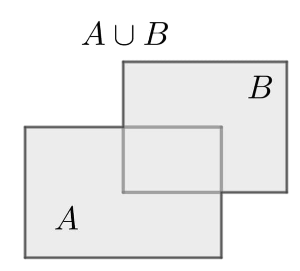
\includegraphics{cup}
\textbf{Пересечением} множеств $A$ и $B$ называется множество, состоящее из элементов принадлежащих как множеству $A$, так и множеству $B$. Обозначается как $A \cap B$.
\\ 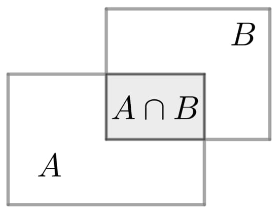
\includegraphics{dasuka}
\textbf{Разностью} множесвом $A$ и $B$ называется множество, состоящее из элементов принадлежащих множеству $A$, но не принадлежащих множеству $B$. Обозначается как $A \setminus B$.
\\ 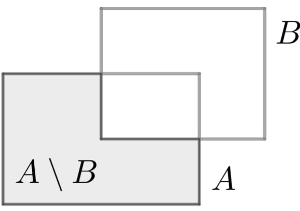
\includegraphics{vichet}
\\И о самом сложном: пусть $A$ и $B$ - множества. Тогда множество $A \times B =^{def} \{ (a, b) | a \in A \wedge b \in B \}$ называется \textbf{декартовым произведением} множества $A$ и $B$ (по картинке правда яснее).
\\ 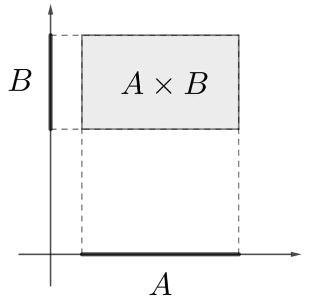
\includegraphics{decart}
Соотвественно, все приведенные выше картинки и есть \textsl{геометрические} смыслы данных операций над множествами; если у вас появились внезапные ассоциации с 9-11 классом и кругами Эйлера - не беспокойтесь, они полностью оправданы, вставьте вместо квадратов круги и грубо говоря будете правы.


\section{Отображение множества $X$ во множество $Y$. Образ и прообраз. Инъективное, сюръективное и биективное отображения. Примеры. Обратное отображение, критерий существования обратного отображения}
\textsl{Презентация по теме: 10.09.24, гл. 1, пар. 4}
\\ \\
\textbf{Отображением} $f$ множества $X$ во множество $Y$ называется правило, сопоставляющее каждому элементу $x \in X$ единственный элемент $y \in Y$. Факт отображения $f$ записывается как $f : X \to Y$ или $X \rightarrow^{f} Y$, а факт \textsl{сопоставления} элемента $x$ элементу $y$ записывается в виде $y = f(x)$ или же $x \to^{f} y$. Внимательные могли заметить что выбор буквы для обозначения отображения и сама формулировка кажется больно знакмой - оно и верно, ибо если $Y = \mathbb{R}$, то $f$ называется \textsl{функцией}.
\\ Пусть $f : X \to Y$ и $E \subset X$. Тогда множество $f(E) =^{def} \{ f(x) | x \in E \}$ называется \textbf{образом} множества $E$ при отображении $f$.
\\ 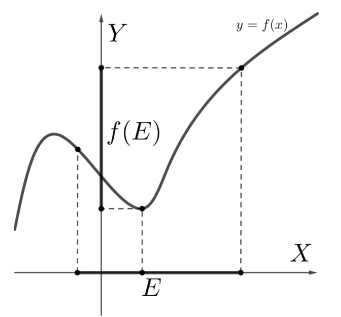
\includegraphics{obraz}
\\ И соотвественно, пусть $f : X \to Y$ и $F \subset Y$. Тогда множество $f^{-1}(F) =^{def} \{ x \in X | f(x) \in F\}$ называется \textbf{прообразом} множества $F$ при отображении $f$.
\\ 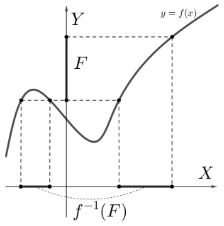
\includegraphics{proobraz}
\\В общем и целом, по-простому, по-людски, так сказать, образ - это множество значений функции от $x$ на некотором участке $E$. Прообраз - обратное действие, дающее значение всех $y$ в неком подмножестве $F$. Геометрические значения даны выше.
\\Отображением $f : X \to Y$ называется \textbf{инъекцией}, если для любых двух различных $x_{1} \in X$ и $x_{2} \in X$ верно то, что $f(x_{1}) \neq f(x_{2})$;  ну или же по более умному: $(\forall (x_{1} \in X \wedge x_{2} \in X) : x_{1} \neq x_{2}) \Rightarrow f(x_{1}) \neq f(x_{2})$
\\Отображение $f : X \to Y$ называется \textbf{сюрьекцией}, если для любого $y \in Y$ найдется $x \in X$ такой, что $f(x) = y$; иначе же - $\forall y \in Y \exists x \in X : f(x) = y$
\\По-простому же - иньекция - это ситуация, при котором для любого $x$ существует собственный \textsl{уникальный} $y$, в то время как сюрьекция - это про то, что для любого $x$ этот самый $y$ \textsl{в целом существует}. В тех случаях же, когда при отображении $f : X \to Y$ выполняются оба правила - такое отображение будет называться \textbf{биекцией}
\\В качестве примера можно просто и незамысловато привести квадратичную функцию $f(x) = x^{2}$ и рассмотреть ее при разных на разных областях определения и значения: так, например, при $X = \mathbb{R}, Y = \mathbb{R}$ не происходит ни сюрьекции, ни иньекции, зато при $X = \mathbb{R}_{+}, Y = \mathbb{R}$ происходит сюрьекция, а при $X = \mathbb{R}_{+}, Y = \mathbb{R}_{+}$ происходит биэкция. Самое сложное во всем этом не путаться между определениями, но с картинками все намного проще\dots
\\Не уверена, будет ли определение композиции отображения, потому на всякий случай замечание - \textbf{композиция отображения} это отображение сложной функции, которое обозначается как $f \circ g(x) =^{def} f(g(x))$. То бишь, $x \rightarrow^{g} y \rightarrow^{f} Z$
\\Пусть $f : X \rightarrow Y$. Отображение $g : Y \rightarrow X$ называется \textbf{обратным отображением} к $f$, если $g(f(x)) = x, \forall x \in X$ и $f(g(x)) = y, \forall y \in Y$. Обратное отображение $g$ обозначается $f^{-1}$ (то есть $f^{-1} = g$). Да, это обратная операция к отображению. Да, как $x \rightarrow^{f} y$, но $y \rightarrow^{f^{-1}} x$. 
\\\textbf{Критерий существования обратного отображения} до ужасного прост - отображение $f : X \rightarrow Y$ должно быть \textsl{биэктивно}. (теорема 4.1)

\section{Конечные, бесконечные, счетные, не более чем счетные и несчетные множества. Примеры}
\textsl{Презентация по теме: 10.09.24, 12.09.24, гл. 1, пар. 5}
\end{document}
